%%%%%%%%%%%%%%%%%%%%%%%%%%%%%%%%%%%%%%%%%%%%%%%%%%%%%%%%%%%%%%%%%%%
%                                                                 %
%                            CHAPTER TWO                          %
%                                                                 %
%%%%%%%%%%%%%%%%%%%%%%%%%%%%%%%%%%%%%%%%%%%%%%%%%%%%%%%%%%%%%%%%%%%

\chapter{ARRAY-BASED MESH REPRESENTATIONS}
\label{chap:struct}

\section{Rationale}

Various requirements for storing of entities, adjacencies,
ability to modify.
Indicate how each requirement affects complexity.

\section{Related Work}

Specifics of mesh representations in the literature.
This can probably come from the SISC paper, plus
some more SCOREC references.

\section{Two Paradigms, Two Structures}

A lead-in describing the two structures and their difference
in abilities.

\section{PUMI/APF Data Structure}

{\color{red} SISC attribution}

\begin{enumerate}
\item The representation centers around graph theoretic interpretations
of topological adjacency.
\item The mesh can remain topologically consistent with and associated with
geometric model entities.
\item The common element types of FE/FV methods can coexist in one structure.
\item Additional data can be associated with entities to implement
high order basis functions, including for geometric approximation.
\item A mesh can be modified by adding and removing single entities in constant time.
\item The entire mesh is stored in a few contiguous dynamic arrays.
\end{enumerate}

One key contribution of this paper is to show that the latter two properties,
array storage and rapid single-entity modification, are not mutually exclusive
and can be combined in a viable way.

{\color{red} BREAK - jump to SISC center}

Given the above discussion of requirements
for finite element mesh information, we now discuss
the common computer representations of unstructured
finite element meshes.

Unstructured mesh applications represent
of the portions of the mesh topology graph
needed to support the operations carried out on the mesh.
A representation which explicitly stores
every entity is said to be a {\it full}
representation.
Any schemes which allow some entities to be represented
implicitly (i.e. their presence does not consume memory)
and be said to be {\it reduced} representations.
We will cover full representations and show that our method
can also produce reduced representations.

Once the set of explicit entities is chosen, one has
options about which adjacencies to store.
Recall from Section \ref{sec:adj} that downward and upward
adjacencies are transitive, so it is enough to
store a subset of the adjacencies such that reachability
remains the same.
One example of this is the {\it one-level} representation,
in which we choose some ordered subset of the dimensions
to explicitly represent and then store the upward
and downward adjacencies between each consecutive
pair of dimensions \cite{beall1997general}.
The full one-level representation, for example, stores
region-face, face-edge, and edge-vertex adjacencies
(both upward and downward).
We will present both full and reduced one-level representations.
Despite this focus on the one-level adjacencies, our structure
in general can be used to store any subset of
adjacency relations.

\begin{figure}
\begin{center}
\includegraphics[width=0.53\textwidth]{full_rep.png}
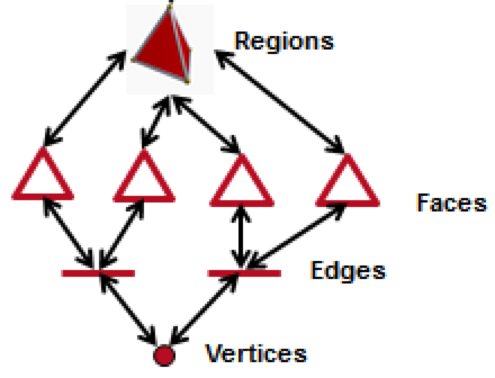
\includegraphics[width=0.4\textwidth]{one_level.png}
\caption{(left) a geometric representation of one-level
relations among a subset of the entities that bound a tetrahedron.
(right) simpler depiction of one-level relations between dimensions}
\label{fig:topo}
\end{center}
\end{figure}

Figure \ref{fig:topo} illustrates the relationships
stored in a full one-level representation.
Each arrow representing an adjacency relation (a.k.a. entity use)
is bi-directional to indicate that we store both the
downward (high to low dimension) and upward (low to high) relations.
Note that vertices are related only to edges,
regions are related only to faces, etc.

A comparison of representations based on the choice
of dimensions and adjacencies between
dimensions to represent
was published by Garimella \cite{garimella2002mesh}.

For any given representation, the computation of $M^d_i\{M^q\}$
can either be done efficiently using stored information
or using an exhaustive search if less information is available.
If a structure can compute $M^d_i\{M^q\}$, where dimensions
$d$ and $q$ are explicitly represented, in constant time,
we say that it is {\it complete} \cite{seol2006efficient}.
Recall from Section \ref{sec:fem} that upward adjacencies
are bound by a constant, so they are computable in
constant-time if enough information is stored.

For general adaptivity,
a complete mesh representation is required to preserve mesh
validity and similarity to the model during edge
collapsing and swapping without imposing additional
restrictions on how coarse the mesh can be.

For most applications, these structures
must also allow the association of user data with any
entities, which is further motivation for storing
all entities, i.e. for a full representation.
Therefore our structure of choice is a full
one-level representation, which means it is also complete.

\subsubsection{Object-Oriented Storage}
\label{sec:sisc_oo}

We begin by describing how our structure would look
if we stored it in an object-oriented manner.
In object-oriented programming, data is organized
into {\it objects} of a few {\it types}.
All objects of the same type have the same {\it attributes},
and for each object and associated attribute a {\it value} must be stored.
In the present case, the objects are mesh topological entities
and the attributes are pointers encoding adjacency relations.

The goal is to organize all data into objects whose
sizes are known at compile time based on their type.
The first step to doing this is to create separate object types
based on topological type.
Objects of the same type are all topologically similar to some polytope,
for example a triangle or a pyramid.
This ensures that their downward adjacency degrees are all the same,
which makes downward adjacency storage fairly straightforward.
For example, a tetrahedron in a full representation would store
four pointers to its bounding faces.

\begin{figure}
\begin{center}
\includegraphics[width=0.9\textwidth]{oo.png}
\caption{(left) the example mesh: a reduced representation of two
triangles sharing one edge and two vertices.
(middle) the linked-list storage of upward adjacency information
for vertices to triangles.
(right) a key describing the meaning of symbols in the middle figure}
\label{fig:oo}
\end{center}
\end{figure}

The second step is to use a linked-list technique \cite{karamete2016novel}
to upward-adjacency storage amongst the entities
of higher dimension, alleviating the need for variable-length
storage in lower-dimensional objects.
If an object stores $m$ downward pointers, then it also stores
$m$ singly-linked list nodes.
A singly-linked list node simply contains a pointer to the next
node, which can also be null.
Every low-dimensional object then stores a single ``head" node
which begins their upward linked list.
If a high-dimensional object ($h$) points to a low-dimensional object ($l$)
from its $j$th downward pointer, then its $j$th list node must be
part of object $l$'s linked list.
Figure \ref{fig:oo} illustrates this portion of the data structure
for a reduced mesh of two triangles.
Notice how, for a shared vertex, one begins at the vertex's head node,
reaches a node that is stored for triangle 0, then continues
to a node stored for triangle 1, which contains a null pointer.
This is fundamentally how upward adjacency is queried for a vertex.
A singly-linked list can be used as opposed to doubly-linked one
because per Section \ref{sec:intro_mesh}
the number of nodes in this list has a constant upper bound.
This means we can afford the $O(m)$ runtime cost of removing a node from this
list when a high-dimensional entity is removed
($m$ being the number of upward adjacent entities),
in exchange for halving the memory use.

\subsubsection{Structure of Arrays}
\label{sec:sisc_soa}

Next we describe how we convert the object-oriented structure
into an array-based one.
Instead of storing all data for a single object contiguously,
i.e. organizing by object first and then by attribute,
we organize data first by attribute and then by object.
We store all data for a single attribute in a contiguous
array, hence this scheme can be called a {\it structure of arrays}
\cite{sung2012dl}.
In our case, examples of attribute arrays would be
the ``first up" nodes for all entities of dimension $d$
and likewise the ``next up" nodes for all entities of dimension $(d+1)$.
For a static mesh we would be done, but this structure needs
to support efficient addition and removal of objects.
We therefore need to manage the arrays which store attributes
for all objects a single type, to account for addition and removal
of objects of that type.

When users request the addition of a new entity, we are allowed
to store it anywhere in the structure.
In this case adding objects in constant time has a well-known
solution called geometric growth \cite{cormen2001table}.
At any time we have some amount of array storage capacity $c(t)$
which is filled entry at a time.
When that storage is full, we reallocate it to a new capacity $c(t+1)$,
such that the integer function $c(t)$ approximates the real function
$f(t) = \alpha^t$, where $1< \alpha\leq 2$.
Although reallocation has a runtime cost of $O(c(t))$, the geometric
growth amortizes this cost such that adding objects
is constant-time on average \cite{cormen2001table}.
The tradeoff is that a bounded fraction of the storage is unused extra space.
In our case, we use a growth formula of $c(t+1) = (3(c(t)+1))/2$
as a heuristic compromise between memory and runtime.

Removing objects is usually the more troublesome operation for
array-based structures.
First, we have no control over which object is being removed.
This means a ``hole" will be created at some arbitrary index.
While some implementations opt to fill this hole immediately
with an existing object, we will avoid this because it requires
changing the index of a live object,
which causes great confusion to users
and leads to programming errors.
We prefer that object indices are like object pointers: constant
throughout the lifetime of the object.
This way a handle/pointer/index may be maintained by the user
and it will have clear meaning even during mesh modification.

If we cannot change indices then the holes must remain, and
we will track them using a free list, or list of available
space \cite{knuth1997list}.
In our implementation, this means creating a new variable array
along with those of the objects.
This array which we call the free list contains pointers
from each hole to the next hole,
and a single head pointer outside this list
points to the first hole.
We can use a singly-linked list efficiently by adding and
removing holes only to and from the front of this list,
both of which are constant-time operations.

In summary, to add an object, we first check whether there
are holes in the free list.
If so, the first hole is used as space for the object,
and it is removed from the free list.
Otherwise the object is added at the end,
which may trigger a geometric growth of all arrays
simultaneously.
To remove an object, we simply add the resulting hole as the first hole
in the free list.
See Figure \ref{fig:flex} for a helpful layout diagram
of modifiable object arrays.

\begin{figure}
\begin{center}
\includegraphics[width=0.8\textwidth]{flex.png}
\caption{Extra space and hole tracking create modifiable arrays}
\label{fig:flex}
\end{center}
\end{figure}

One issue with this structure is that memory use does
not decrease immediately when removing objects, and in theory we can
only shrink the arrays if the last object is removed.
This is connected to our decision to preserve identifiers,
and can be fixed by temporarily relaxing that constraint.
In a single collective step, all objects can be reordered,
given new identifiers, and all links between them updated
accordingly.
If the new identifiers are contiguous, the arrays can shrink
to minimal size.
Beyond that, we can choose a reordering which
makes subsequent queries cache-friendly.
Beall and Shephard describe a reordering for mesh entities which
improves the locality of subsequent adjacency queries
and, more importantly, the sparsity pattern of
matrices assembled from finite element meshes \cite{beall1997general}.
Adjacency-based reordering was expanded upon and
tested by Zhou et al. \cite{zhou2010adjacency}.
This is a supported operation in our implementation,
which combines hole removal with adjacency-based reordering
that improves locality.

An important benefit of this array-based structure is the
ease with which additional attributes can be added or removed
at runtime.
To add a new attribute to objects of the same type, we just
create a new array and ensure that subsequent resizing
operations apply to that array along with the others.
For example, different simulations may require different
attributes such as position, velocity, mass, and electrical charge.
These can each be allocated as a separate array,
and each can be added and removed at runtime as needed
with essentially no memory overhead.

\subsubsection{Lists in Arrays}
\label{sec:lia}

Since our initial structure composed of many small objects containing pointers
to one another was recast into a set of large arrays
as opposed to individually allocated objects,
pointers to objects get transformed into array indices.
As an example, consider the transformation for a singly-linked
list as shown in Figure \ref{fig:arraylist}.

All the list nodes are packed into an array, and a pointer to
a list node becomes an index into this array, starting with zero.
Since zero is a valid index, we can use -1 to denote a null pointer.
Notice also that if we have knowledge about the maximum length
of the array, we can choose an integer type that uses less bytes
than a pointer, since pointers must be able to index the entire
virtual address space.

\begin{figure}
\begin{center}
\includegraphics[width=0.6\textwidth]{arraylist.png}
\caption{(left) A linked list in object form, each node containing
a memory address pointer to the next node.
(right) The same linked list packed into an array.
The data contained inside each node is the array index of the next node.
Underneath each node, its own index is indicated.
The letters serve to indicate corresponding nodes before and after.}
\label{fig:arraylist}
\end{center}
\end{figure}

Since indices can have the same meaning for several arrays,
we can separate the variables in an object into different
arrays.

\subsubsection{Dynamically Modifiable Mesh Structure}
\label{sec:sisc_mstruct}

\begin{figure}
\begin{center}
\includegraphics[width=0.95\textwidth]{mixed.png}
\caption{(left) an example subset of a mixed mesh:
an edge adjacent to a triangle and a quad.
(right) the corresponding upward adjacency linkage
must traverse separate triangle and quad arrays.}
\label{fig:mixed}
\end{center}
\end{figure}

There is one more detail that needs resolving in the
case of mixed meshes.
The problem is that different polytope
groups may contain uses of the same entity.
For example, an edge may be used by a triangle and a quadrilateral.
They must be linked together, but their arrays are
separated by polytope group.
In order to be able to jump between those arrays, we must
enhance the indices being used.
Our solution is to encode information about the polytope group
into these indices, i.e. $e = (t,i)$ where $t$ is an integer
uniquely identifying a polytope group, $i$ is the index
into the arrays of that group, and $e$ is the extended index.
In particular, the encoding we choose is $e = iT + t$, where
$T$ is the total number of polytope groups and $0\leq t < T$.
This allows the extended index to remain an integer
and be decoded using simple modulo and division instructions.
Figure \ref{fig:mixed} illustrates this representation.
Starting with entry $20$ in the ``edge first up" array,
we are directed to edge use $2$ of quad $10$.
At entry $i=(10\cdot 4 + 2)$ of the ``quad next up" array,
we are further directed to edge use $0$ of triangle $4$.
At entry $i=(4\cdot 3 + 0)$, we find a null pointer and stop.

To get clear picture of all the arrays and their groupings
that are allocated for a real mesh, here is a listing
including all polytope types that a complex CFD mesh
might need when boundary layers are constructed with
a mix of wedges and pyramids:
\begin{enumerate}
\item Vertices
  \begin{enumerate}
  \item Coordinates (size $=3\times$vertex capacity)
  \item First edge (size $=$vertex capacity)
  \item Free list (size $=$vertex capacity)
  \end{enumerate}
\item Edges
  \begin{enumerate}
  \item Vertices used (size $=2\times$edge capacity)
  \item Next edge up (size $=2\times$edge capacity)
  \item First face up (size $=$edge capacity)
  \item Free list (size $=$edge capacity)
  \end{enumerate}
\item Triangles
  \begin{enumerate}
  \item Edges used (size $=3\times$triangle capacity)
  \item Next face up (size $=3\times$triangle capacity)
  \item First region up (size $=$triangle capacity)
  \item Free list (size $=$triangle capacity)
  \end{enumerate}
\item Quadrilaterals
  \begin{enumerate}
  \item Edges used (size $=4\times$quadrilateral capacity)
  \item Next face up (size $=4\times$quadrilateral capacity)
  \item First region up (size $=$quadrilateral capacity)
  \item Free list (size $=$quadrilateral capacity)
  \end{enumerate}
\item Tetrahedra
  \begin{enumerate}
  \item Faces used (size $=4\times$tetrahedra capacity)
  \item Next region up (size $=4\times$tetrahedra capacity)
  \item Free list (size $=$tetrahedra capacity)
  \end{enumerate}
\item Wedges
  \begin{enumerate}
  \item Faces used (size $=5\times$wedges capacity)
  \item Next region up (size $=5\times$wedges capacity)
  \item Free list (size $=$wedges capacity)
  \end{enumerate}
\item Pyramids
  \begin{enumerate}
  \item Faces used (size $=5\times$pyramid capacity)
  \item Next region up (size $=5\times$pyramid capacity)
  \item Free list (size $=$pyramid capacity)
  \end{enumerate}
\end{enumerate}
Where the capacities refer to the geometric growth
capacity described in Section \ref{sec:sisc_soa} based
on the current number of entities of that polytope group.

This structure provides a straightforward mechanism for associating
data with each entity of a polytope group by creating
new arrays as described in Section \ref{sec:sisc_soa}.
This is how vertex coordinates and entity-level fields
are stored.


\section{Omega\_h Data Structure}

\subsection{Adjacency Cache}

\subsection{Alignment Codes}

\section{Data Structure Performance}

Query times, modification times, etc. for both structures.

%%% Local Variables:
%%% mode: latex
%%% TeX-master: t
%%% End:
